\chapterimage{addb4870c144badba811c06724df8512.jpg}
\chapter{Anexos}
\section{Código}
\subsection{Patrón Fachada}
%\begin{figure}[H]
%	\centering
%	\includegraphics[width=0.5\linewidth]{codfachada1}
%	\centering
%	\caption{Interfaz monitoría (fachada)}
%	\label{fig:codfachada1}
%\end{figure}
\clearpage
\begin{figure}[H]
	\centering
	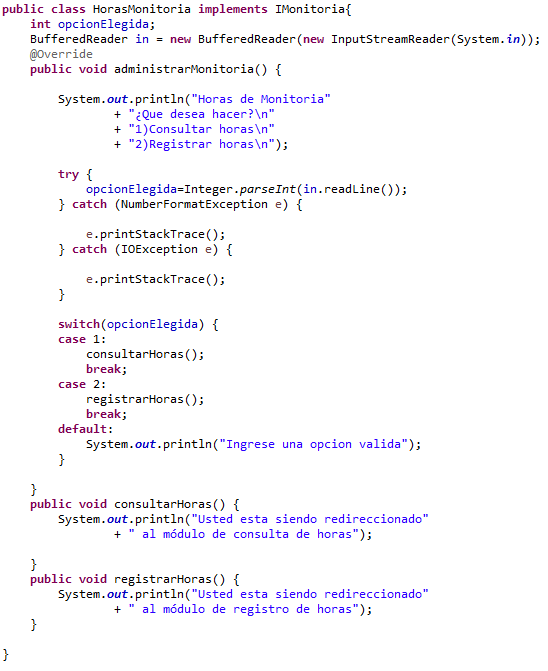
\includegraphics[width=1\linewidth]{codfachada2}
	\centering
	\caption{Ejemplo de implementación para la fachada}
	\label{fig:codfachada2}
\end{figure}
\begin{figure}[H]
	\centering
	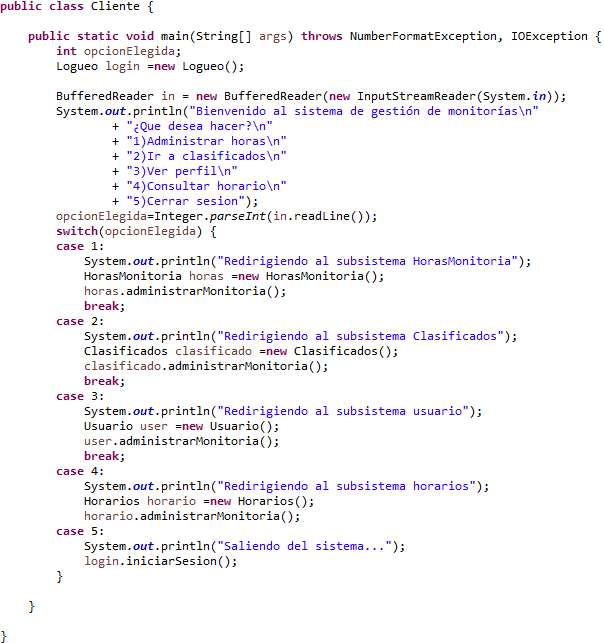
\includegraphics[width=1\linewidth]{codfachada3}
	\centering
	\caption{Cliente ejemplo fachada}
	\label{fig:codfachada3}
\end{figure}
\subsection{Patrón Proxy}
\begin{figure}[H]
	\centering
	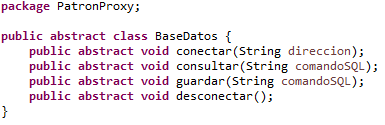
\includegraphics[width=0.5\linewidth]{codproxy1}
	\centering
	\caption{Clase abstracta de las bases de datos}
	\label{fig:codproxy1}
\end{figure}
\clearpage
\begin{figure}[H]
	\centering
	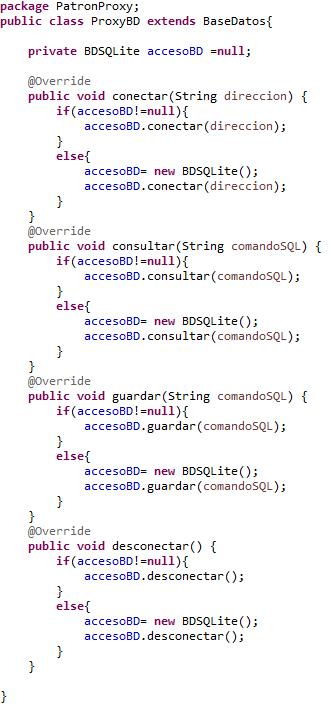
\includegraphics[width=0.7\linewidth]{codproxy2}
	\centering
	\caption{Clase proxy para el manejo de la conexión en SQLite}
	\label{fig:codproxy2}
\end{figure}
\begin{figure}[H]
	\centering
	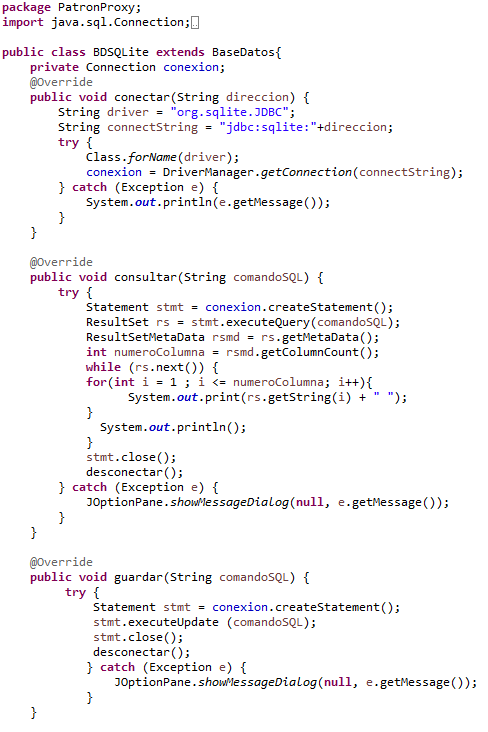
\includegraphics[width=1\linewidth]{codproxy3}
	\centering
	\label{fig:codproxy3}
\end{figure}
\begin{figure}[H]

	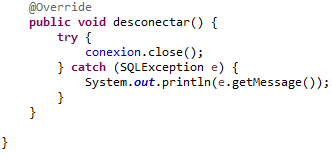
\includegraphics[width=0.7\linewidth]{codproxy4}
	\caption{Clase con la lógica de la base de datos para SQLite}

\end{figure}
\begin{figure}[H]
	\centering
	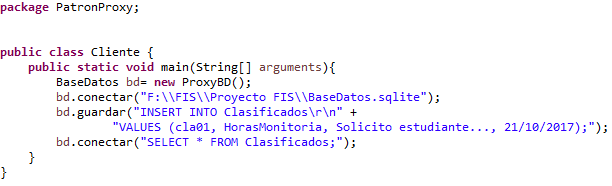
\includegraphics[width=1\linewidth]{codproxy5}
	\centering
		\caption{Cliente con un ejemplo de implementación}
	\label{fig:codproxy5}
\end{figure}

\subsection{Patrón Comando}
\begin{figure}[H]
	\centering
	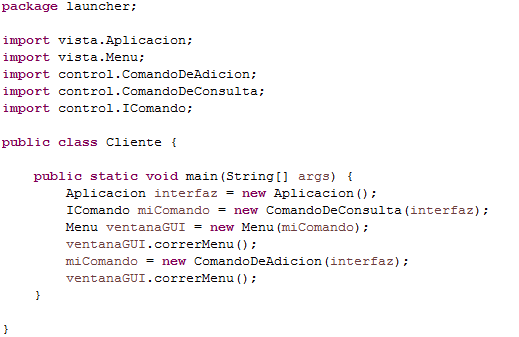
\includegraphics[width=0.5\linewidth]{codComando1}
	\centering
	\caption{Clase Cliente que ejecuta el comando}
	\label{fig:codComando1}
\end{figure}
\clearpage
\begin{figure}[H]
	\centering
	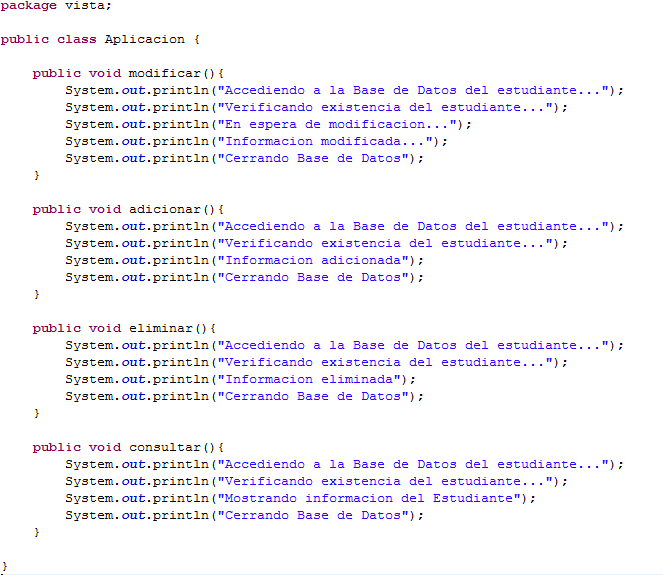
\includegraphics[width=0.7\linewidth]{codComando2}
	\centering
	\caption{Clase Aplicacion donde se manejan las consultas a la BD}
	\label{fig:codComando2}
\end{figure}
\begin{figure}[H]
	\centering
	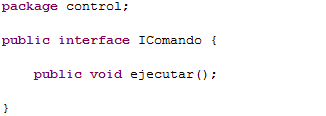
\includegraphics[width=1\linewidth]{codComando3}
	\centering
	\caption{Interface comando}
	\label{fig:codComando3}
\end{figure}
\begin{figure}[H]
	\centering
	\caption{Implementación de la interfaz comando por cada metodo de Aplicacion}
	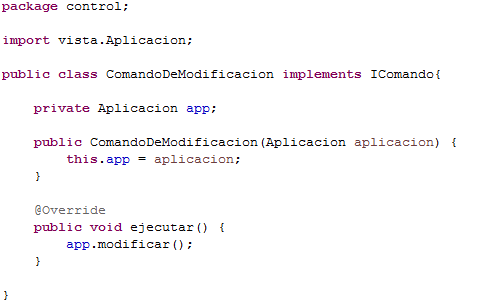
\includegraphics[width=1\linewidth]{codComando4}
	\caption{Comando de Modificación}
	\centering
	\label{fig:codComando4}
\end{figure}
\begin{figure}[H]
	\centering
	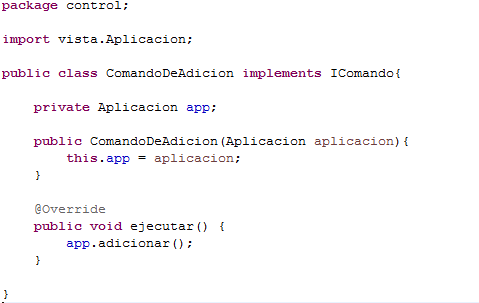
\includegraphics[width=1\linewidth]{codComando5}
	\centering
	\caption{Comando de Adición}
	\label{fig:codComando5}
\end{figure}
\begin{figure}[H]
	\centering
	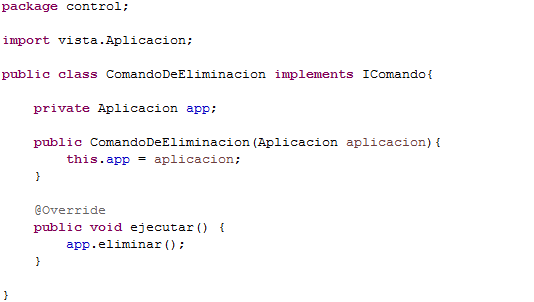
\includegraphics[width=1\linewidth]{codComando6}
	\centering
	\caption{Comando de Eliminación}
	\label{fig:codComando6}
\end{figure}
\begin{figure}[H]
	\centering
	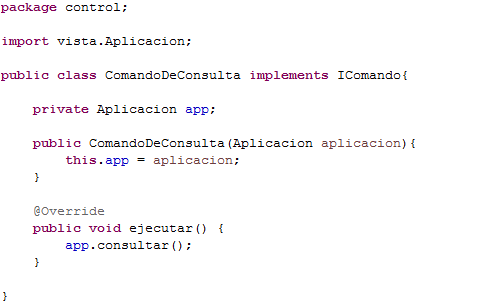
\includegraphics[width=1\linewidth]{codComando7}
	\centering
	\caption{Comando de Consulta}
	\label{fig:codComando7}
\end{figure}
\begin{figure}[H]
	\centering
	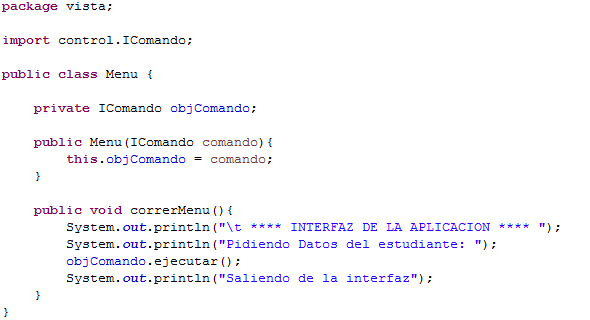
\includegraphics[width=1\linewidth]{codComando8}
	\centering
	\caption{Clase Menu con la que interactua el cliente en la GUI}
	\label{fig:codComando8}
\end{figure}

\subsection{Patrón Singleton}

\begin{figure}[H]
	\centering
	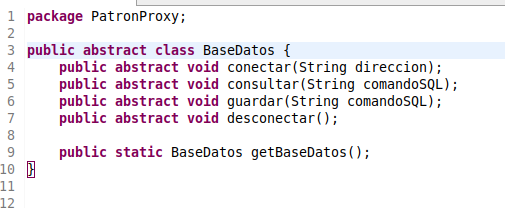
\includegraphics[width=1\linewidth]{codSingleton}
	\centering
	\caption{Clase abstracta BaseDatos, parte del patrón proxy, con singleton implementado}
	\label{fig:codSingleton}
\end{figure}
\begin{figure}[H]
	\centering
	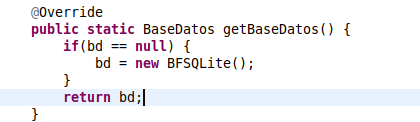
\includegraphics[width=1\linewidth]{codSingleton1}
	\centering
	\caption{Clase BDSQLite, parte del patrón proxy, con singleton implementado}
	\label{fig:codSingleton1}
\end{figure}
\begin{figure}[H]
	\centering
	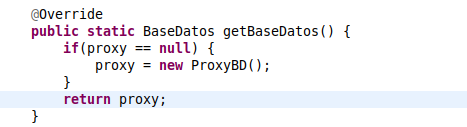
\includegraphics[width=1\linewidth]{codSingleton2}
	\centering
	\caption{Clase ProxyBD, parte del patrón proxy, con singleton implementado}
	\label{fig:codSingleton2}
\end{figure}

\subsection{Patrón Componente}
\begin{figure}[H]
	\centering
	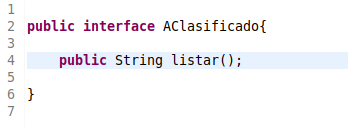
\includegraphics[width=1\linewidth]{codComposite}
	\centering
	\caption{Clase AClasificado, contiene interfaz que implementan los clasificados}
	\label{fig:codSingleton2}
\end{figure}
\begin{figure}[H]
	\centering
	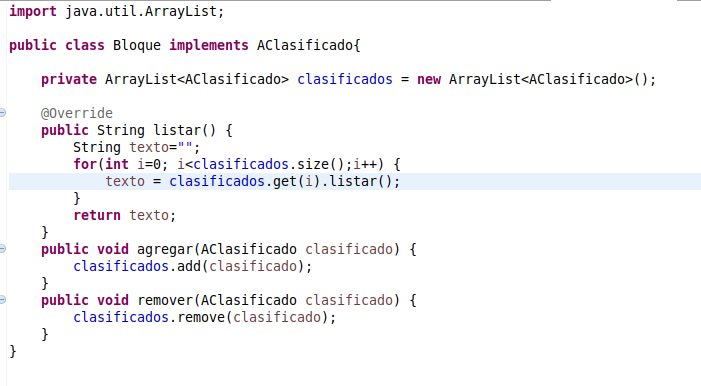
\includegraphics[width=1\linewidth]{codComposite1}
	\centering
	\caption{Clase Bloque, contiene los objetos tipo clasificados}
	\label{fig:codSingleton2}
\end{figure}
\begin{figure}[H]
	\centering
	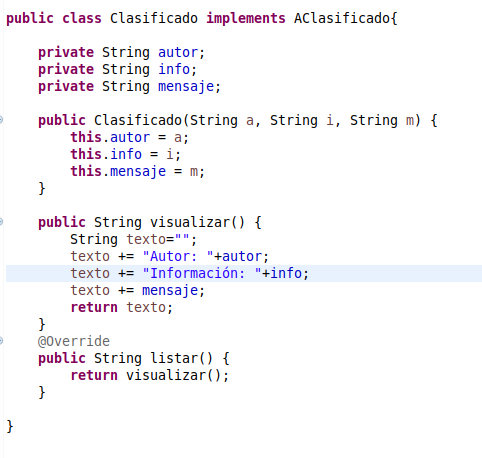
\includegraphics[width=1\linewidth]{codComposite2}
	\centering
	\caption{Clase Clasificado}
	\label{fig:codSingleton2}
\end{figure}